\documentclass[12pt, a4paper]{article}
\usepackage[utf8]{inputenc}
\usepackage{hyperref}
\usepackage{graphicx}
\usepackage{listings}
\usepackage{xcolor}
\usepackage{float}

\definecolor{codegreen}{rgb}{0,0.6,0}
\definecolor{codegray}{rgb}{0.5,0.5,0.5}
\definecolor{codepurple}{rgb}{0.58,0,0.82}
\definecolor{backcolour}{rgb}{0.95,0.95,0.92}

\lstdefinestyle{mystyle}{
    backgroundcolor=\color{backcolour},   
    commentstyle=\color{codegreen},
    keywordstyle=\color{magenta},
    numberstyle=\tiny\color{codegray},
    stringstyle=\color{codepurple},
    basicstyle=\ttfamily\footnotesize,
    breakatwhitespace=false,         
    breaklines=true,                 
    captionpos=b,                    
    keepspaces=true,                 
    numbers=left,                    
    numbersep=5pt,                  
    showspaces=false,                
    showstringspaces=false,
    showtabs=false,                  
    tabsize=2
}

\lstset{style=mystyle}

\hypersetup{
    colorlinks=true,
    linkcolor=black,
    urlcolor=cyan,
}

\graphicspath{{img/}}


\title{\textbf{Elaborato di Intelligenza Artificiale} \\ Implementazione di una Simulazione con Modelli di Reti Neurali Utilizzando l'Ambiente di Sviluppo Python}
\author{Soldà Matteo --- 1226319}
\date{\today}

\begin{document}

\begin{figure}
    \centering
    \includegraphics[width=0.50\textwidth]{Logo_Università_Padova}
\end{figure}

\maketitle

\newpage
\begin{abstract}
Nel presente elaborato verrà implementata una simulazione tramite modelli di reti neurali utilizzando l'ambiente di sviluppo Python.\\
La simulazione si baserà sul database \textit{MNIST}, riguardante il riconoscimento di numeri manoscritti, fornitoci durante la terza esercitazione pratica.\\
Dopo aver introdotto i vari tipi di rete e i loro risultati tramite un breve report, si cercherà rispondere a tre domande essenziali: definire le cifre più difficili da riconoscere, quantificare la variazione di accuratezza dovuta all'inserimento di rumore nel \textit{training pattern} e la variazione dell'accuratezza di riconoscimento sul \textit{testing pattern} riducendo drasticamente le dimensioni del \textit{training pattern}.    
\end{abstract}

\newpage
\tableofcontents

\newpage
\section{Introduzione}
In questo elaborato si prenderà in considerazione uno dei problemi più famosi che vengono sottoposti alle intelligenze artificiali: il riconoscimento di numeri manoscritti.
La simulazione chè verrà presentata si baserà sul dataset \textit{MNIST}, il quale contiene 70.000 immagini, con relative etichette, di cifre comprese tra 0 e 9 scritte a mano.\\
Per risolvere il problema sopra descritto, utilizzeremo due Percettroni Multi-Strato: la variante classica e quella convoluzionale.\\
Per testare entrambe le reti, suddivideremo il dataset in due parti: il training set composta da 60.000 immagini e il test set composto da 10.000 immagini. Dopo l'addestramento della rete, si procederà con la predizione, per poi passare ad una seconda predizione nel quale il test set conterrà del rumore crescente.

\newpage
\section{Costruzione della Rete Neurale e Test --- Breve Report}
\subsection{Multi Layer Perceptron --- Versione Classica}
Come prima rete, è stata creata un Percettrone Multi-Strato composto da 500 strati nascosti, ognuno dei quali formato da 500 neuroni. Effettuato l'addestramento su un massimo di 15 cicli e tramite funzione di attivazione "\textit{RELU}", la curva di apprendimento appare come sotto riportato:
\begin{figure}[H]
    \centering
    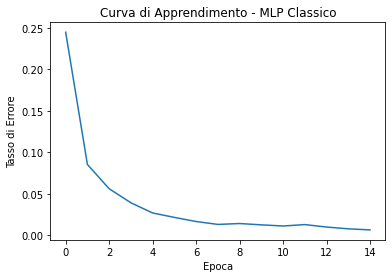
\includegraphics[width=0.50\textwidth]{Curva_MLP}
\end{figure}
Tramite la funzione \textit{score()}, si calcola che l'accuratezza della rete è fissata a \(97.79\%\).
Per completezza, è stato anche effettuato una predizione sullo stesso test set dove sono stati inseriti, in diversi step, 10 livelli di rumore compresi nell'intervallo \([0.1 , 1.0]\). Di seguito la variazione dell'errore all'aumentare del rumore:
\begin{figure}[H]
    \centering
    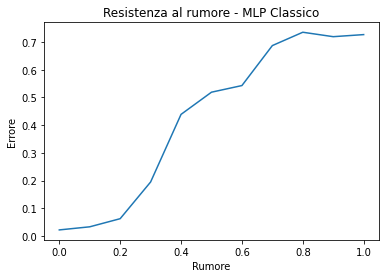
\includegraphics[width=0.50\textwidth]{Rumore_MLP.png}
\end{figure}

\subsection{Multi Layer Perceptron --- Versione Convoluzionale}
A seguire, è stata creata una variante convoluzionale di MLP formata da 2 strati convoluzionali così definiti:
\begin{itemize}
    \item Primo Strato: 18 filtri e un kernel \(3*3\)
    \item Secondo Strato: 28 filtri e un kernel \(4*4\)
\end{itemize}
Entrambi questi strati presentano una funzione di attivazione "\textit{RELU}".\\
Dopo aver addestrato la rete, la curva di apprendimento risulta essere:
\begin{figure}[H]
    \centering
    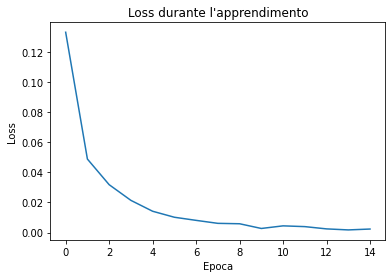
\includegraphics[width=0.50\textwidth]{Curva_Conv.png}
\end{figure}
Tramite la funzione di predizione abbiamo potuto constatare che l'accuratezza risulta essere del \(99.91\%\).\\
Anche in questo caso è stato effettuato il test su vari livelli di rumore e l'accuratezza al variare del rumore risulta essere:
\begin{figure}[H]
    \centering
    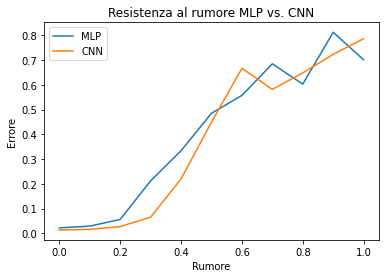
\includegraphics[width=0.50\textwidth]{Rumore_Conv.png}
\end{figure}

\subsection{Risultati}

\newpage
\section{Primo Quesito --- Numeri Difficili da Riconoscere}
\subsection{Visualizzazione di Pattern Erronei}
\subsection{Aggiunta di Rumore in Pattern Corretti}
\subsection{Visualizzazione di Pattern Erronei con Aggiunta di Rumore}

\newpage
\section{Secondo Quesito --- Variazione dell'Accuratezza su Addestramento Rumoroso}
\subsection{Accuratezza su di un Pattern di Test dopo Addestramento Rumoroso}
\subsection{Definizione di un Valore di Rumorosità Ottimale}

\newpage
\section{Terzo Quesito --- Variazione dell'Accuratezza su Pattern di Addestramento Ridotto}
\subsection{50\% del Training Set}
\subsection{25\% del Training Set}
\subsection{10\% del Training Set}


\end{document}
